\documentclass{amsart}
\usepackage{array}
\usepackage{multicol}
\usepackage{longtable}
\usepackage{subfig,enumerate}
\usepackage{ragged2e, color}
\usepackage{amsmath,amssymb,amsthm,graphicx, graphics}
\usepackage[all]{xy}
\usepackage[pdfpagelabels]{hyperref}                 % For creating hyperlinks in cross references

\usepackage{pgf,tikz}
\usepackage{mathrsfs,multicol}

\usepackage[absolute,overlay]{textpos}
\usetikzlibrary{arrows}

%CALCULUS
\newcommand{\dydx}{\frac{dy}{dx}}
\newcommand{\ddx}{\frac{d}{dx}}
\newcommand{\ddt}{\frac{d}{dt}}
\newcommand{\dd}[2]{\frac{d#1}{d#2}}
\newcommand{\uv}{\vec{u}}
\newcommand{\vv}{\vec{v}}
\newcommand{\wv}{\vec{w}}
\newcommand{\av}{\vec{a}}
\newcommand{\bv}{\vec{b}}
\newcommand{\rvt}{\vec{r}(t)}
\newcommand{\rvtp}{\vec{r}\,'(t)}
\newcommand{\vvp}{\vec{v}\,'(t)}
\newcommand{\uvp}{\vec{u}\,'(t)}
\newcommand{\fv}[1]{\langle #1 \rangle} 
\newcommand{\ihat}{\mathbf{\hat{\textbf{\i}}}}
\newcommand{\jhat}{\mathbf{\hat{\textbf{\j}}}}
\newcommand{\khat}{\mathbf{\hat{\textbf{k}}}}
\newcommand{\la}{\left\langle\,}
\newcommand{\ra}{\,\right\rangle}
\newcommand{\dotp}{\hspace{.25em}\begin{picture}(-1,1)(-1,-3)\circle*{2}\end{picture}\hspace{.5em} }
\newcommand{\proj}[2]{\textrm{proj}_{\,#2}\:#1 }
\newcommand{\compp}[2]{\textrm{comp}_{\,#2}\:#1 }
\newcommand{\pder}[2]{\frac{\partial #1}{\partial #2}}
\newcommand{\ppder}[3]{\frac{\partial^2 #1}{\partial #3\,\partial #2}}
\newcommand{\V}[1]{\vec{#1}}
\newcommand{\ds}{\displaystyle}
\newcommand{\curl}{\mathrm{curl}\,}
\renewcommand{\div}{\mathrm{div}\,}

%STANDARD SETS
\newcommand{\R}{\mathbb{R}}
\newcommand{\Q}{\mathbb{Q}}
\newcommand{\Z}{\mathbb{Z}}
\newcommand{\C}{\mathbb{C}}
\newcommand{\N}{\mathbb{N}}
\newcommand{\F}{\mathbb{F}} %finite field

%GENERAL
\newcommand{\inv}{^{-1}}
\newcommand{\del}{\partial}
\newcommand{\by}{\times}

\newcommand{\comp}{\circ}

\newcommand{\infunion}{\bigcup_{i=1}^\infty}
\newcommand{\infcap}{\bigcap_{i=1}^\infty}
\newcommand{\floor}[1]{\lfloor #1 \rfloor}

\newcommand{\blankline}{\vspace{.1in}}
\newcommand{\fillin}[1]{\underline{\hspace{#1 in}}}


\parindent 1cm
\parskip 0.2cm
\topmargin -1.5cm

\oddsidemargin -1cm
\evensidemargin -1cm
\textwidth 18.5cm
\textheight 23.5cm
\newtheorem{theorem}{Theorem}
\newtheorem{proposition}[theorem]{Proposition}
\newtheorem{corollary}[theorem]{Corollary}
\newtheorem{lemma}[theorem]{Lemma}
\newtheorem{remark}[theorem]{Remark}



\theoremstyle{definition}
\newtheorem{formula}[theorem]{Formula}
\newtheorem{example}{Example}
\newtheorem{definition}{Definition}

\begin{document}

\section*{Region 1}


Set up all six orders of integration for \[\iiint\limits_{R_1} f(x,y,z) \, dV\] where $R_1$ is the region bounded by the planes \[y=0, \ z=0, \ x=2, \ y=x, \text{and} \ z=x+y\]

\begin{figure}[!ht]
	\centering
	\begin{tabular}{m{6cm}m{6cm}}%{cc}
		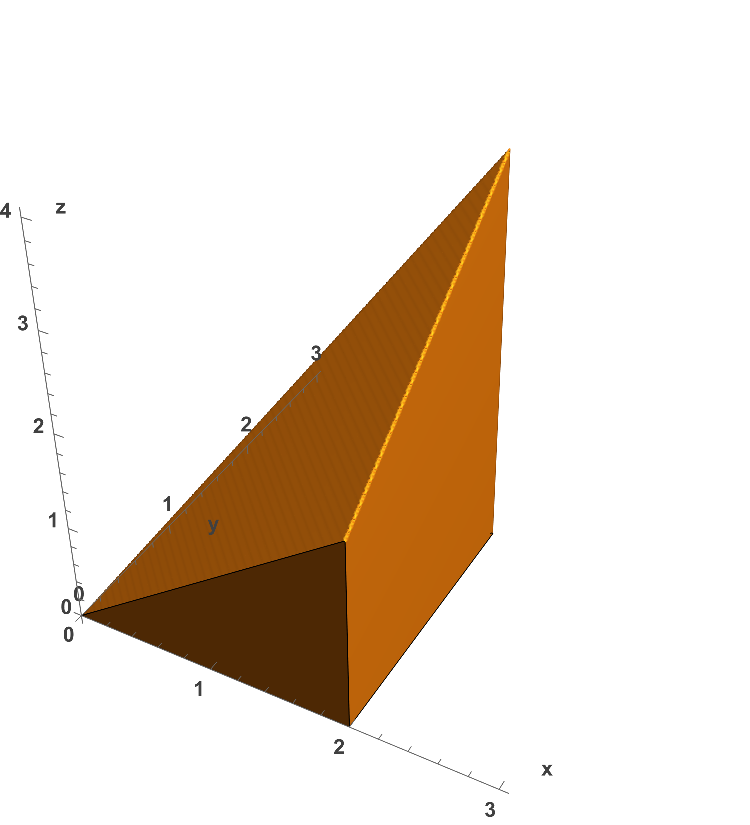
\includegraphics[width=0.4\textwidth]{Region1_Mathematica.pdf} &
		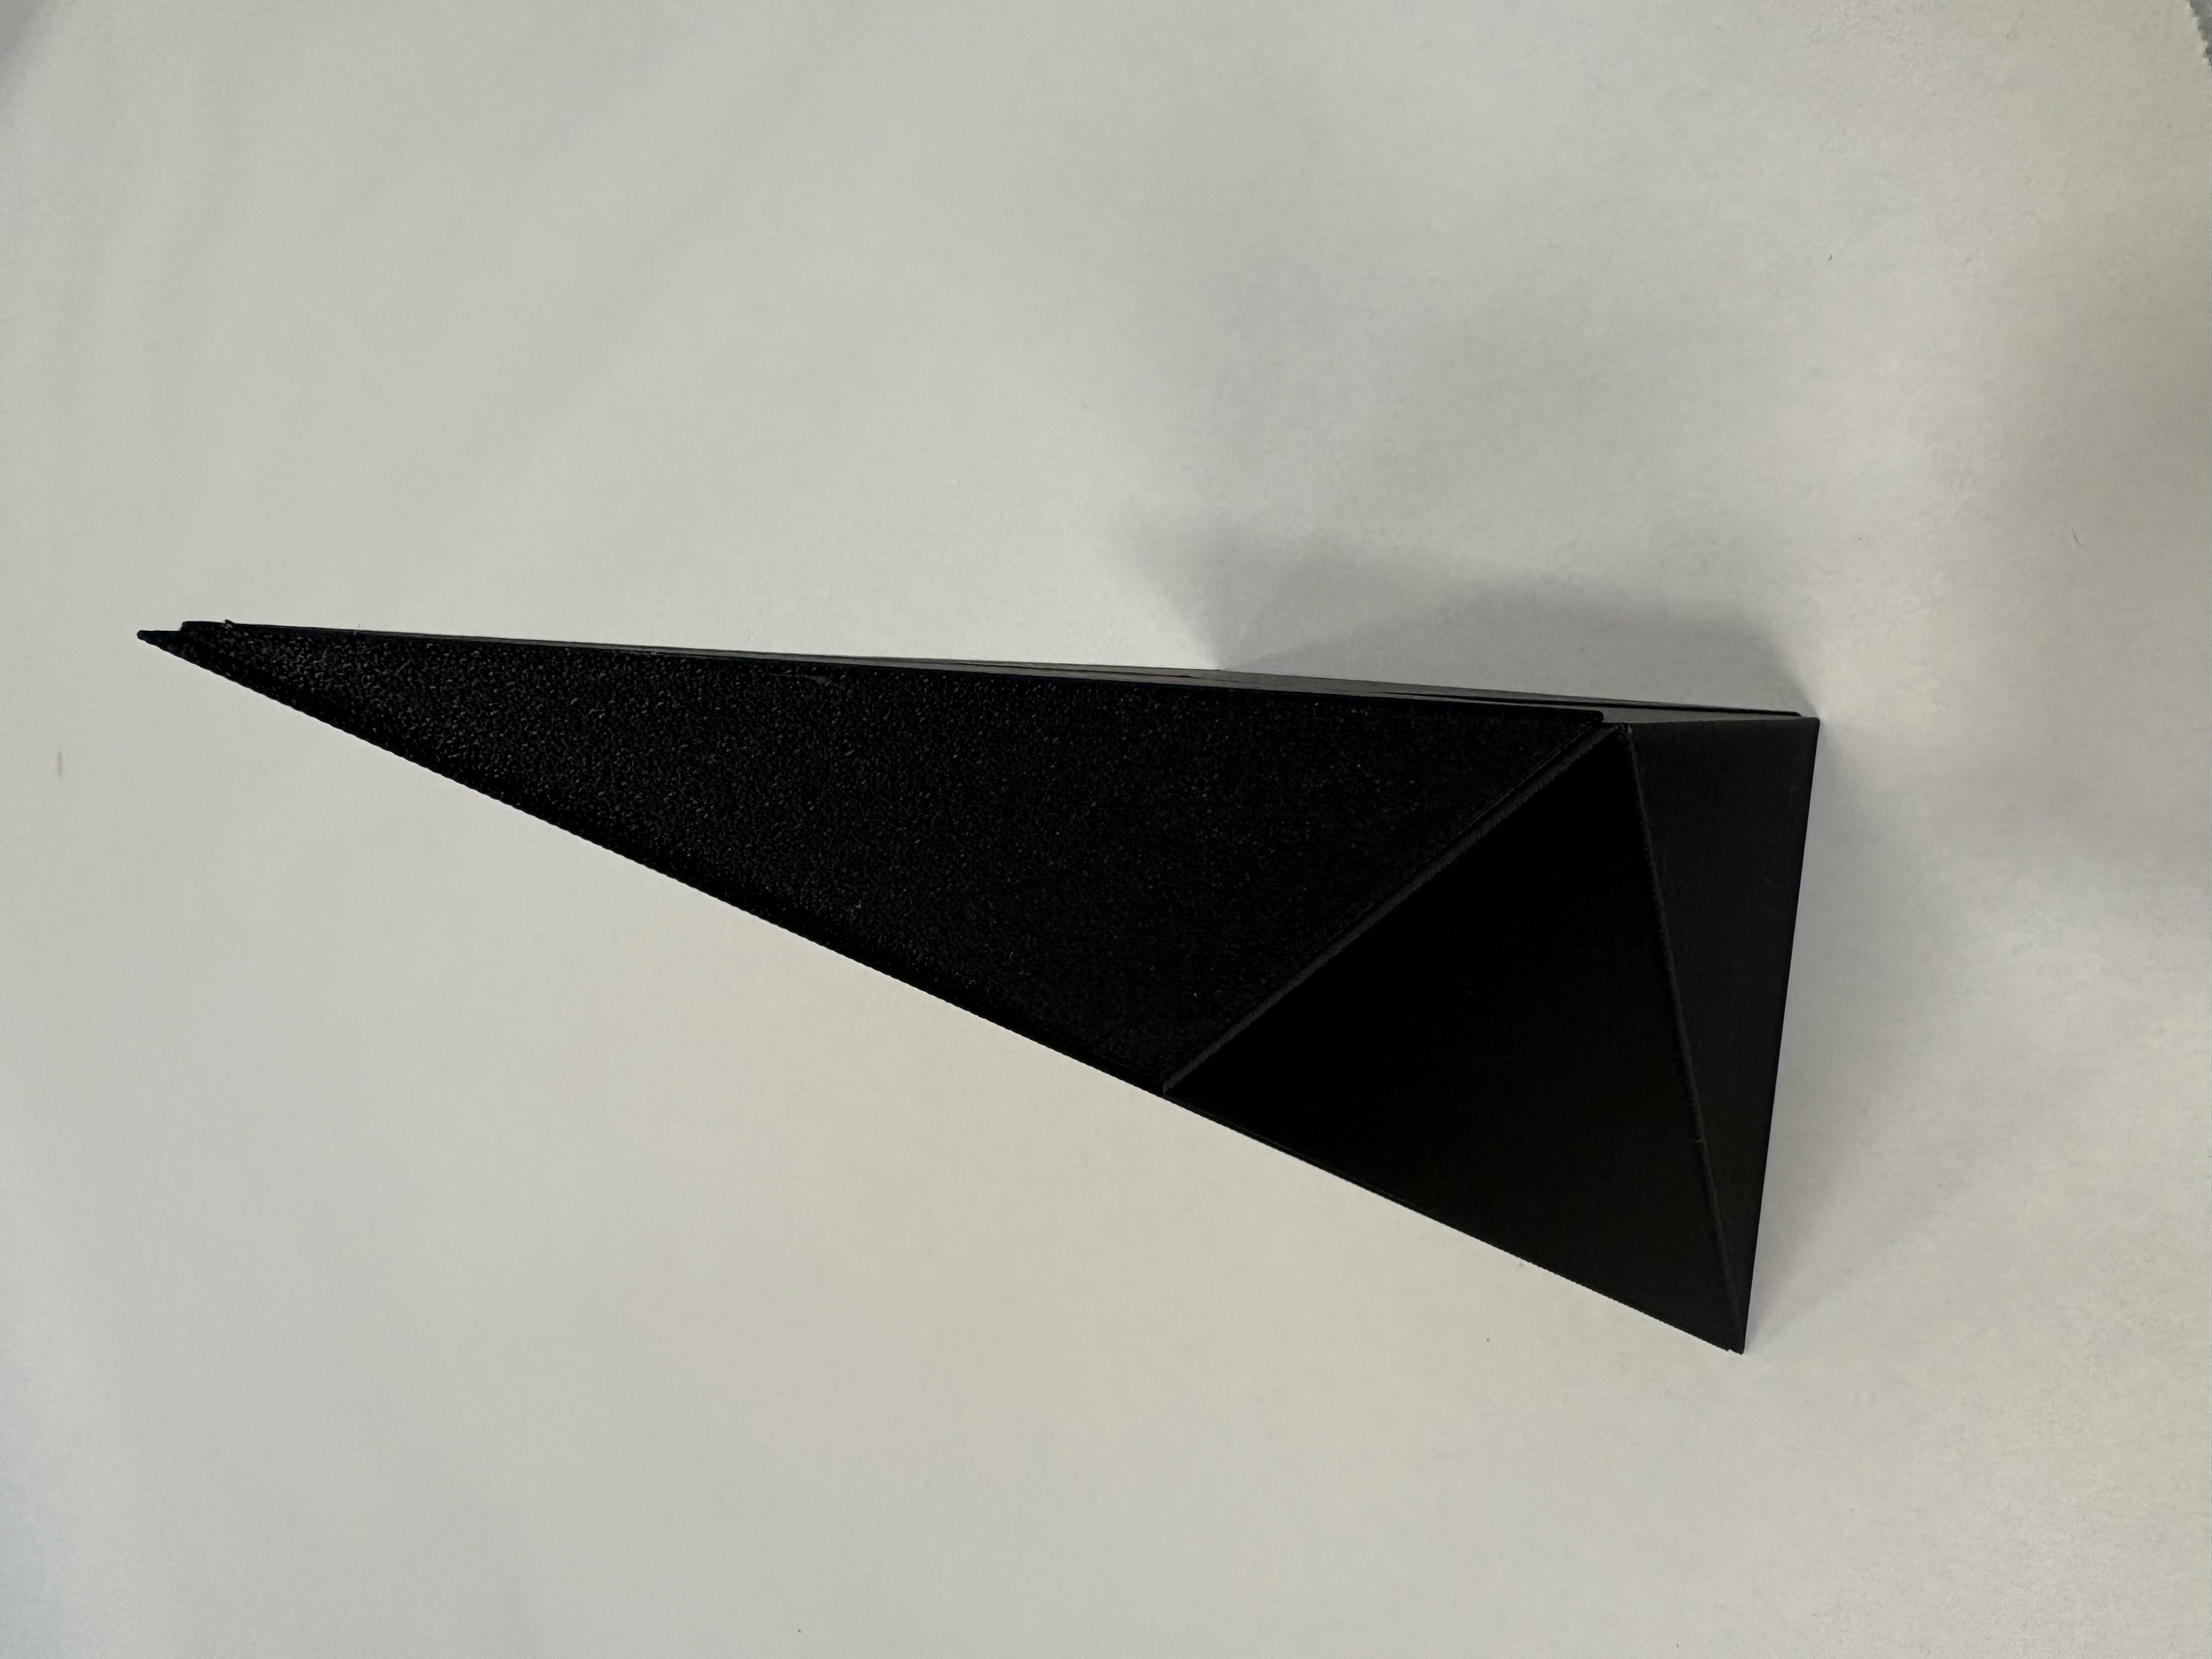
\includegraphics[width=0.45\textwidth]{Solid1Print}
	\end{tabular}
	\caption{Computer-modeled and 3D-printed views of $R_1$.}
\end{figure}

\begin{figure}[!ht]
	\centering
	\begin{tabular}{ccc}
		\subfloat[$xy$-projection.]{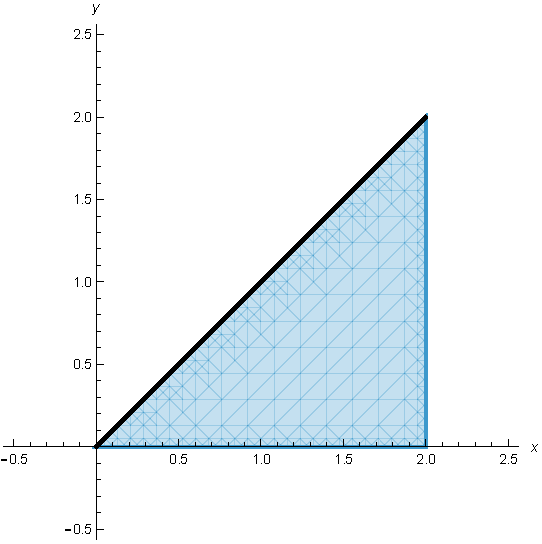
\includegraphics[width=.3\textwidth]{region1_view1.pdf}} &
		\subfloat[$xz$-projection.]{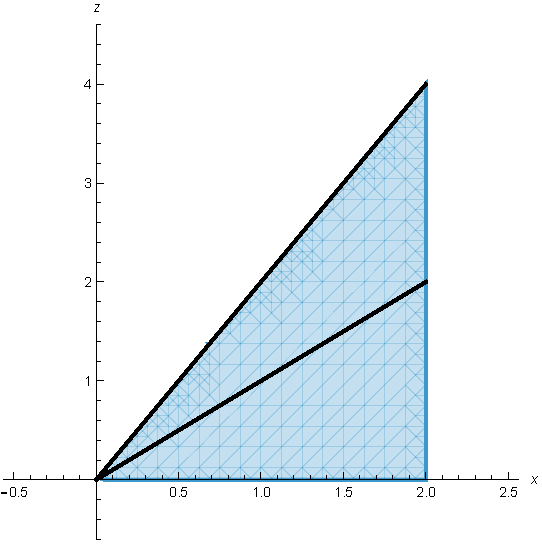
\includegraphics[width=.3\textwidth]{region1_view2.pdf}} &
		\subfloat[$yz$-projection.]{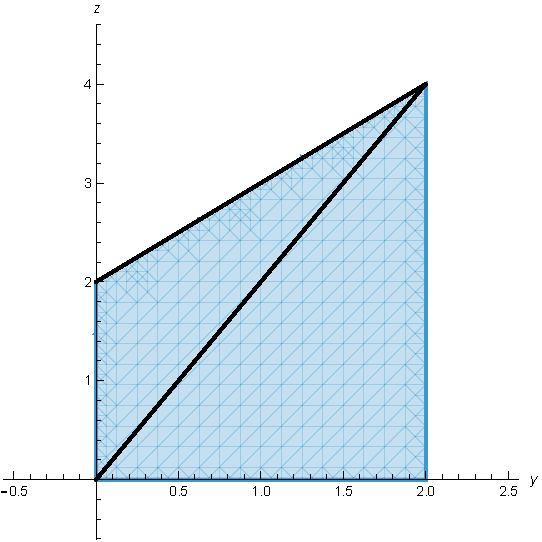
\includegraphics[width=.3\textwidth]{region1_view3.pdf}}
	\end{tabular}
	\caption{Projections of $R_1$ into the three coordinate planes.}\label{projE1}
\end{figure}

\clearpage
~
\vspace{1em}
The following triple integrals represent integrating over the region using the $xy$-projection:
\vspace{0.5cm}
\[\int_0^2\int_0^x\int_0^{x+y} \ f(x,y,z) \ dz \, dy \, dx \]
\vspace{0.5cm}
\[\int_0^2\int_y^2\int_0^{x+y} \ f(x,y,z) \ dz \, dx \, dy \]

\vspace{0.5cm}
The following triple integrals represent integrating over the region using the $xz$-projection:
\vspace{0.5cm}
\[\int_0^2\int_0^{x}\int_0^{x} \ f(x,y,z) \ dy \, dz \, dx \ + \ \int_0^2\int_x^{2x}\int_{z-x}^{x} \ f(x,y,z) \ dy \, dz \, dx \]
\vspace{0.5cm}
\[\int_0^2\int_z^{2}\int_0^{x} \ f(x,y,z) \ dy \, dx \, dz \ + \ \int_0^2\int_{\frac{z}{2}}^{z}\int_{z-x}^{x} \ f(x,y,z) \ dy \, dx \, dz \ + \ \int_2^4\int_{\frac{z}{2}}^{2}\int_{z-x}^{x} \ f(x,y,z) \ dy \, dx \, dz \]

\vspace{0.5cm}
The following triple integrals represent integrating over the region using the $yz$-projection:
\vspace{0.5cm}
\[\int_0^4\int_{\frac{z}{2}}^{2}\int_{y}^{2} \ f(x,y,z) \ dx \, dy \, dz \ + \ \int_0^2\int_0^{\frac{z}{2}}\int_{z-y}^{2} \ f(x,y,z) \ dx \, dy \, dz \ + \ \int_2^4\int_{z-2}^{\frac{z}{2}}\int_{z-y}^{2} \ 1 \ dx \, dy \, dz \]
\vspace{0.5cm}
\[ \int_0^2\int_0^{2y}\int_{y}^{2} \ f(x,y,z) \ dx \, dz \, dy \ + \ \int_0^2\int_{2y}^{y+2}\int_{z-y}^{2} \ f(x,y,z) \ dx \, dz \, dy \]

\vspace{1em}
All of these triple integrals evaluate to $4$ when $f(x,y,z) = 1$.

\end{document}



























